% --------------------------------------------------------------------

\section{Introduction}

The first stage of committing a cyber attack or a penetration test is reconnaissance or a network footprinting. The aim of reconnaissance is to acquire information about the target network infrastructure. Various footprinting techniques may be used to query publicly available data, such as using advanced search features of search engines and WHOIS queries. One such technique is Domain Name System (DNS) enumeration which uses public DNS records to gather information about the target without actually probing the target network. The Domain Name System may reveal information such as IP addresses, domains, subdomains, mail exchange services and services.

Objective of this thesis is to conduct a literary review about the existing DNS enumeration techniques and their operating principles and related security enhancements that has been made to DNS.

The goals of this thesis is as follows:

\begin{itemize}
 \item Conduct a literary review about existing DNS enumeration techniques
 \item Discuss modifications that have been made to the Domain Name System to implement security
 \item Present some use cases of the existing methods.
\end{itemize}

DNS has been and still is vulnerable to attacks such as DNS cache poisoning where the attacker tricks a DNS server or a resolver to store false information in a DNS cache e.g., to route a client to a phishing site. DNS Security Extensions or DNSSEC has been developed to prevent cache poisoning attacks but the way DNSSEC is implemented has opened up new ways to conduct DNS enumeration. Therefore DNSSEC will be discussed but DNS cache poisoning attacks are out of the scope of this study. In addition recent developments in DNS and enumerating cloud services are briefly discussed.


\section{The Domain Name System}

The Domain Name system or DNS \cite{RFC1035}\cite{RFC1034} is a fundamental part of the Internet infrastructure. This chapter gives a brief overview of DNS, related security issues and recent developments related to this study.

\subsection{Overview}
Domain Name System is a distributed database implemented in a hierarchy of DNS servers with delegated authority that stores information about services and other resources on the Internet. Notably, DNS stores information that maps host names to IP addresses. The Domain Name System as a whole consists of specification for the functionality of DNS servers and the DNS protocol. The DNS protocol for DNS queries is for the most part based on the UDP protocol. DNS protocol is part of the Internet Protocol Suite and as an application layer protocol is commonly employed by other application layer protocols such as HTTP, SMTP or FTP to resolve domain names to IP addresses. \citep{kurose_ross}\cite{tanenbaum} 

When an application makes a query to retrieve an IP address for a host name, the corresponding IP address is resolved in an iterative manner by a DNS resolver. For most Internet users DNS resolver is a service provided by Internet Service Provider. From an application perspective query is executed in a recursive manner, see Figure \ref{fig:resolving}.  

At the top level of the name server infrastructure there are 13 logical root name servers distributed across the globe named from A to M. If an answer for a query is not found in cache of the resolver a root name server is queried first which delegates the query for a top level domain such as .com., to a Top Level Server Domain server or TLD server. The iteration continues until an Authoritative Name Server is found for the host. The query result is returned to the client via DNS resolver. \citep{kurose_ross} \cite{tanenbaum} 

There is another class of DNS servers called a local or private DNS Server which is strictly not part of the DNS hierarchy, but is part of the DNS infrastructure. A private DNS server may be used in a private network. \citep{kurose_ross}


\begin{figure}[htb]
  \begin{center}
    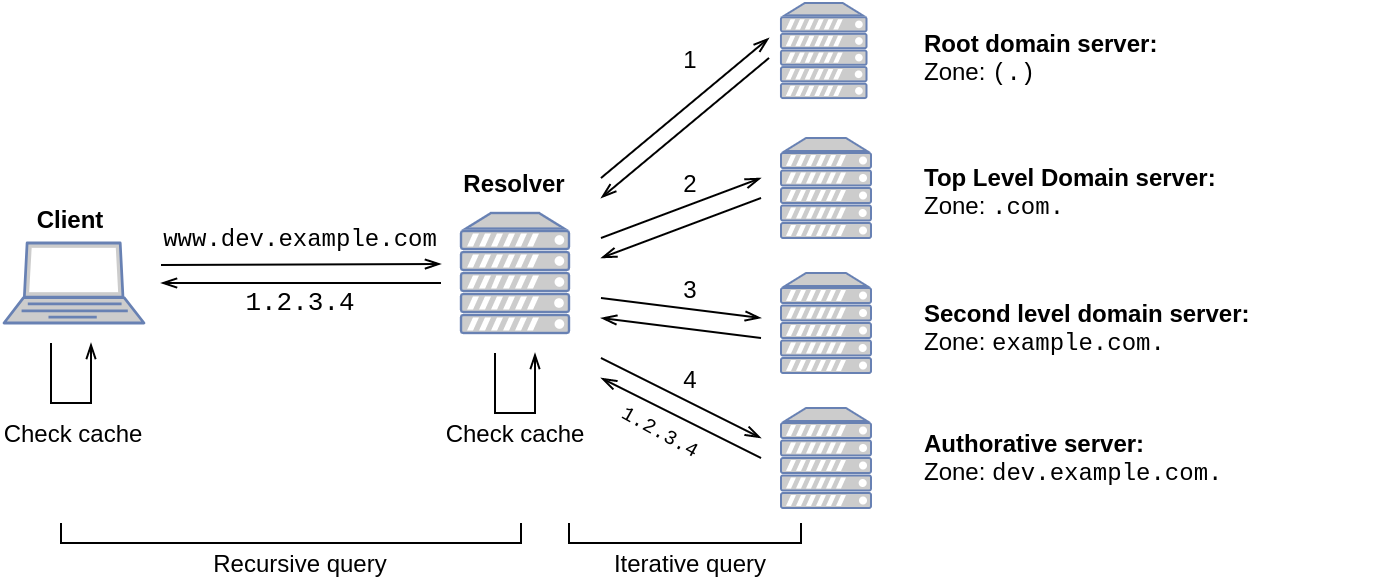
\includegraphics[width=0.9\textwidth]{resolving2.png}
    \caption{A simplistic presentation of resolving an IP address for a host \texttt{www.dev.example.com}. An Iterative query is performed by the DNS resolver until an authoritative name server for subdomain \texttt{dev.example.com} is found. The authoritative server has a type A resource record which maps the name \texttt{www.dev.example.com} into an IP address. Explanation for zones, see Section \ref{sec:dns_zones}.}
    \label{fig:resolving}
  \end{center}
\end{figure}

\subsection{DNS Resource Record Types}

A DNS database or a DNS record has multiple queryable resource record types. Most common and relevant for this study are listed in Figure \ref{table:dns_record_types}. Among A and AAAA records,  PTR record has a special interest related to this study since it allows reverse DNS lookup which maps an IP address to a hostname. Main uses for PTR records are anti-spam filtering and logging \cite{PTR_uses}. NSEC and NSEC3 resource records can be used to execute an enumeration method called Zone Walking as is discussed later on.

\begin{table}[th]
\caption{Most common or most the relevant DNS Record types for this study.}
\label{table:dns_record_types}
\begin{center}
\begin{tabular}{|p{0.35\textwidth}|p{0.45\textwidth}|} 
    \hline
Record Type & Description \\
    \hline
    \hline
A & IPv4 address for a host. \cite{RFC1035}\\ 
    \hline
AAAA & IPv6 address for a host \cite{RFC3596}\\
    \hline
MX & Mail exchange server. \cite{RFC1035} \\
    \hline
CNAME & Canonical Name. Maps an "alias" to a canonical name. \cite{RFC1035} \\
    \hline
SOA & Start of Authority. Specifies authoritative information about a DNS zone, including the primary name server for the zone. \cite{RFC1035}\\    \hline
PTR & A Pointer Record. Maps an IP address to a hostname. \cite{RFC1035} \\
    \hline
    
NSEC & Provides an authenticated denial of
   existence for DNS Resource Record Sets. Points to a next Domain in canonical order. \cite{RFC3845}. 
\\
\hline
NSEC3 & Similar to NSEC but hashed values of domain names are used instead of plain text. \cite{RFC5155} \\
\hline

NSEC3PARAM & Holds cryptographic information related to NSEC3. \cite{RFC5155}\\
\hline

RRSIG & Resource record signature for a resource record set. \cite{RFC4034}\\
\hline

SRV & Specifies hostname and port number of servers for specified services. \cite{RFC2782}\\
\hline


\end{tabular}
\end{center}
\end{table}


\subsection{DNS Zones}
\label{sec:dns_zones}

A DNS zone is a distinct part of domain namespace which is delegated to an entity such as an organization. DNS zones should not be associated with domain namespaces, meaning there is no one to one correspondence between a zone and a domain. A single DNS server may be responsible for multiple zones, and for replication, load distribution and security (e.g., to deflect DDoS attacks) there are usually multiple domain name servers for each zone. \citep{tanenbaum}

In the example presented in Fig. \ref{fig:resolving} second level domain name server for \texttt{example.com} has delegated the responsibility of subdomain \texttt{dev.example.com} for another zone.

If there are multiple domain name servers for a zone there is a primary DNS server which is replicated by secondary servers. A secondary DNS server maintains a read-only copy of the DNS zone file maintained in the primary DNS server. If modifications are made they are made into the DNS zone file of the primary DNS server. The process of secondary DNS server requesting an update and receiving this information is called a Zone Transfer. \citep{tanenbaum}

\subsection{Publicity and Security of DNS}
\label{sec:dns_security}


The intrinsic property of DNS records is that they are public by design and normal DNS queries are not encrypted. In the initial design of DNS there were no security features implemented. The DNS system has a long history of being vulnerable for DNS spoofing, also referred to as DNS cache poisoning, where the attacker tricks a DNS server to store false information in a DNS cache. \cite{tanenbaum}\cite{RFC_threat_analysis} 

DNS Security Extension or DNSSEC (defined originally in now obsolete \cite{RFC_2065}) has been developed to provide end-to-end data integrity and source authenticity check between the source of DNS data and the client. To achieve this, DNSSEC uses public/private key pair signatures (RRSIG resource record). Threaths of data disclosure were ruled out of scope of DNSSEC \cite{RFC_threat_analysis}. Although DNSSEC was standardized already in 1997 it is still not widely used but the adoption is slowly progressing \cite{lotr}. In 2013 ICANN started a process of approving new TLDs with the additional requirement that they are secured by DNSSEC \cite{sweden}. DNSSEC relies on authentication chain of trust. All root level domain name servers use DNSSEC signatures, but if a TLD does not implement DNSSEC there can not be DNSSEC for any domain under such TLD since the chain of trust is broken \cite{lotr}.

Transmission signatures or TSIG \cite{RFC_2845_trans_sec} use shared private keys to provide authentication of servers to secure actions such as zone transfers and dynamic updates of resource records.


\subsection{Recent developments in DNS}

Even though DNS was initially designed to translate domain names to IP addresses, the DNS has evolved into a complex system and has many uses beyond its original intent. A common dns query for example for \texttt{TXT} resource records reveal much information such as Google site verification and whitelisting email for spam verification. In the current form DNS may even be considered to be a distributed key value database for myriad of applications.

Currently, DNSSEC provides data integrity and source authenticity, but DNS lacks confidentiality since DNS queries and responses are visible to network elements on the path. In recent years new standards for encrypting DNS query traffic has been proposed such as DNS over TLS [RFC 7858], DNS Queries over HTTPS [RFC 8484] and DNS over Datagram Transport Layer Security [RFC 8094]. 

For some domains, it can be desirable to provide web sites or other services at a bare domain name, such as \texttt{domain.com} instead of \texttt{www.domain.com}. Use of CNAME record type for this purpose is in conflict with DNS specifications. RFC 1034 \cite{RFC1034} states that if there is a CNAME RR in a zone for a name there can not be any other RR for that name in the zone. If the zone is a so-called apex zone i.e., the zone contains SOA and NS resource records for the domain name, according to \cite{RFC1034} use of CNAME for the domain name in this zone is prohibited. To overcome this limitation some managed DNS providers such as Route 53 by Amazon \cite{Route53}, DNSimple \cite{DNSimple} and ClouDNS \cite{ClouDNS} use a non-standard ALIAS resource record that can coexist with other resource records for a name. The ALIAS record is not returned to a DNS resolver but is resolved instead internally by the DNS server into an IP address to achieve compliance with DNS specifications. Due to use of a non-standard ALIAS resource record by multiple DNS providers a standard for new resource record (ANAME) with similar functionality is being developed \cite{ANAME}.

As internet services are moving to the cloud, websites are turning to Content Delivery Networks (CDN) to provide services. CDNs are dynamic and change IP addresses based on the users' location and server load. Instead of static DNS records managed DNS providers nowadays use an anycast network and provide dynamic DNS records with features such as geolocation, failover and even load balancing on a DNS level \cite{ManagedDNS}.
% 7858 = prevent eavesdropping
% 8484 = security for integrity and confidentiality
% 8094 =  DNS queries and responses are visible to network elements on the path
% between the DNS client and its server.
\section{DNS Enumeration}

Due to the original design philosophy and easy access principle, DNS is vulnerable to information leakage and attacks such as DNS cache poisoning. Since DNS records are public DNS queries allow attackers the gather information about the target networks using various methods of DNS Enumeration such as using a dictionary attack to enumerate subdomains. DNS Enumeration is part of the reconnaissance stage where an attacker gathers information about the target network. DNS enumeration includes gathering information about IP addresses, domains and subdomains.

DNS Enumeration is considered to be part of the Open Source Intelligent or OSINT methodology where publicly available (open source) information is used in an intelligence context \cite{network_sec_assessment}. DNS enumeration is commonly used jointly with other OSINT methods such as \texttt{whois} queries and exploiting advanced search engine features such as "Google Dorks" \cite{network_sec_assessment}.

This chapter will review the most common methods of DNS enumeration and in the last section (\ref{sec:cloud}) cloud services are briefly discussed.

\subsection{Basic DNS lookup}

Every resource record or RR can be considered a five-tuple (Name, Type, Class, Time to Live, Value) \cite{RFC1035}. Some of the Types were listed in Table \ref{table:dns_record_types}. In addition to Types (TYPE), DNS defines query types (QTYPE) which is a superset of types. The DNS protocol also defines a query class (QCLASS) as a superset of class (CLASS). Every query contains QNAME (fully qualifed domain name or FQDN), QTYPE and QCLASS \cite{RFC1035}.

\texttt{Nslookup} and 'Domain Internet Grober' (\texttt{dig}) are common tools found in most Unix enviroments to carry out basic DNS queries. For example \texttt{dig -q www.example.com -t AAAA -c IN} returns an IPv6 address for \texttt{www.example.com} with query class \texttt{IN} (Internet). In practise the query class is now redundant since the query class \texttt{IN} is the only one in use but is required by the protocol definition.

Above example which returns an IP address for a host name is called a forward lookup. A reverse lookup is a query returning a host name for an IP address (PTR record).

\subsection{Zone Transfer Attack}

As explained in Section \ref{sec:dns_zones} each DNS zone is composed by a primary server and secondary servers. Secondary servers maintain read-only copies of the primary servers zone file. DNS protocol defines a special type of query, Asynchronous Transfer Full Range or AXFR which requests for a transfer of an entire list of resource records for zone or a Zone File \cite{RFC1034}. The DNS zone information may include sensitive information e.g., the internal infrastructure of a network of an organization. If a DNS server is misconfigured, the attacker may retrieve the zone file from a DNS server. The zone file is a plain text list of all resource records of the zone.

Although succeeding in unauthorized zone transfer requests is considered by some as a thing for the past \cite{network_sec_assessment}, on a global-scale vulnerability assessment  \citet{global_zone_transfer} were able to carry out approximately 11 million zone transfers containing information such as HINFO (information about OS and CPU \cite{RFC1035}) records, and domains with \texttt{test.} and \texttt{dev.} prefixes etc.

The AXFR offers no authentication mechanism \cite{RFC1035}\cite{RFC5936}. In order to prevent the vulnerability from occurring the DNS server should be configured to only allow AXFR requests from trusted IP addresses. Additionally the use of TSIG or SIG(0) are recommended for authentication of trusted servers\cite{RFC5936}. Since AXFR uses TCP \cite{RFC1034}\cite{RFC1035} a firewall could be configured to block TCP traffic to port 56 for untrusted clients but since DNS queries over 512 bytes will be transferred over TCP this is not practical \cite{hacking_exposed}.


%subsection{Zone Enumeration}


%Another vulnerability related to our work is so-called zone
%enumeration. Initially, ability to enumerate all the names in
%a zone was not considered as an error [2], however, later on,
%a compromise has been reached [22] that in certain cases,
%the knowledge of all the domain names in a zone can lead
%to security risks. RFC 5155 [22] provides some examples
%showing that due to this vulnerability, it is easier for an attacker
%to obtain email addresses for future spam campaigns or data
%useful during a reconnaissance phase of a network attack."  \citet{global_zone_t
%ransfer}


\subsection{Reverse DNS sweeping}

Once IP address ranges used by the target are discovered one can use reverse DNS sweeping. IP network blocks can be discovered for example using whois queries or other reconnaissance methods (see e.g., \cite{network_sec_assessment}) or even by an educated guess. Reverse DNS sweeping in itself is quite a simple method. Reverse DNS queries are performed for a range of IP addresses. 

As an example DNS forward lookup reveals four A resource records for domain \texttt{hs.fi}:
\begin{verbatim}
---
;; ANSWER SECTION:
hs.fi.			60	IN	A	13.32.143.49
hs.fi.			60	IN	A	13.32.143.98
hs.fi.			60	IN	A	13.32.143.126
hs.fi.			60	IN	A	13.32.143.119
---
\end{verbatim}
One can infer (or quess) that maybe there is a reserved IP block, \texttt{13.32.143.0/24}. Reverse sweep can be executed for example using \texttt{nmap} tool:
\begin{verbatim}
> nmap -sL 13.32.143.0/24 | grep "13" | awk '{printf("%s %s\n",$5,$6);}'

server-13-32-143-0.hel50.r.cloudfront.net (13.32.143.0)
server-13-32-143-1.hel50.r.cloudfront.net (13.32.143.1)
...
server-13-32-143-254.hel50.r.cloudfront.net (13.32.143.254)
server-13-32-143-255.hel50.r.cloudfront.net (13.32.143.255)
\end{verbatim}

From the domain names one can infer that the service is provided by Amazon Web Services content delivery network. Further investigation reveals that ip addresses are for Cloudfront edge servers \cite{AWS}.

\subsection{Zone Enumeration}

DNSSEC introduced the ability for a hostile party to enumerate all names in a zone. Initially, ability to enumerate all the names in a zone was not considered as an error but was recognized as a drawback of DNSSEC \cite{RFC_4033}.

As explained in section \ref{sec:dns_security} the purpose of DNSSEC is to provide end-to-end data integrity and source authenticity check in the Domain Name System. This section will not cover DNSSEC in detail but an important part of DNSSEC which is called an authenticated denial of 
of existence in DNS  \cite{RFC_7129}. The section will further discuss how the authenticated denial of existence can be leveraged to execute a DNS enumeration technique called Zone Walking or Zone Enumeration.

\subsubsection{Denial of Existence in DNS}

DNSSEC signatures are used only for signing the Resource Records in the DNS response message or packet. The DNS message header is not signed. \citep{RFC_7129}  

The DNS response message header contains a status code. If a DNS query is made for an existing name (QNAME), status code of the response header is NOERROR and the answer section contains Resource Records for the name in question, which are signed if DNSSEC is supported. 
There are two cases of status codes corresponding to situations where requested Resource record does not exits \cite{RFC_7129}:

\begin{itemize}
 \item If a query is made for a name that does not exist the status code of the response is \texttt{NXDOMAIN} (Non-Existing Domain).  
 \item If a query is made for a name that does exist but the requested resource record does not exist the status code of the response is \texttt{NOERROR}. Based on the response the resolver can infer that the type of response is of type called \texttt{NODATA}.
\end{itemize}

Since DNSSEC signature is not used to sign DNS message header the NXDOMAIN status cannot be trusted. In addition the DNSSEC signatures are precomputed. The original design of DNSSEC excluded online signing due to security reasons (to keep the private key offline) and the computational overhead. Therefore, offline signing the header is not feasible since it would require precomputing signatures for all conceivable nonexisting answers. \citep{RFC_7129}

Above elaborates the issue with DNSSEC and authenticated denial of existence: if an empty answer is returned there are no resource records to sign. The first attempt to specify authenticated denial of existence was NXT resource record. NXT was introduced in \cite{RFC_2065} but has been superceded by NSEC resource record \cite{RFC3845}.

NSEC resource record indirectly lets the resolver know that the name does not exist in the zone. Zone is sorted into canonical order and NSEC describes an interval between names \cite{RFC4034}. For example if a zone contains domain names \texttt{a.domain.org} and \texttt{c.domain.org} and in canonical ordering there are no domain names in between in the zone, DNS query for a domain name \texttt{b.domain.org} returns (class and time to live omitted for simplicity):

\begin{verbatim}
Name	            Type    Value
a.domain.org     NSEC    c.domain.org NS SOA TXT RRSIG NSEC DNSKEY
\end{verbatim}

The answer above is returned since \texttt{b.domain.org} resides in the interval between \texttt{a.domain.org} and \texttt{c.domain.org}. The value returned contains the endpoint of the interval and a list of resource records types where RRSIG, NSEC and DNSKEY are related to DNSSEC. NSEC records are signed as are other resources in DNSSEC. 

NSEC records are also used in \texttt{NODATA} responses as is explained in \citep{RFC_7129}.


\subsubsection{Zone Walking}

The drawback of NSEC is that it permits DNS enumeration method called Zone Walking or Zone Enumeration. An enumerated zone can be used, for example, as a source of open mail servers for spam. NSEC records point from one name to another and this allows enumeration of the whole zone thus defeating attempts to block zone transfers. An attacker can query these NSEC RRs in sequence to obtain all the names in a zone. \citep{RFC3550} \citep{hacking_exposed} \citep{RFC_7129} 

For example using \texttt{dig} tool it is easy to see if a top level domain uses NSEC. In the example below one can see that when that when making a DNS query for a TLD name server (\texttt{a.fi}) responsible for top level domain \texttt{fi.}, the authority section reveals that NSEC3 is used for denial of existence, see section \ref{sec:nsec3}. Dig tool offers an option \texttt{+dnssec} which sets the \texttt{DO} bit ("\texttt{DNSSEC OK}") to inform a DNS server that the client is DNSSEC-aware [RFC4035].


\begin{verbatim}
> dig +dnssec @a.fi fi.
---
;; AUTHORITY SECTION:
---
uhirv2ck3kkgn20e3fnqecj1nfu6eeko.fi. 86400 IN NSEC3 1 1 5 7B7EE2F28EAFC626
 UHKSO58SOE3BAFENJNSU6QKL13RGLTP4
---
\end{verbatim}

In the previous result \texttt{uhirv2ck3kkgn20e3fnqecj1nfu6eeko} is the hash value for \texttt{fi.}, \texttt{7B7EE2F28EAFC626} a salt used in hashing and \texttt{UHKSO58SOE3BAFENJNSU6QKL13RGLTP4} the next hash value for a domain in the canonical list of hashes. The number of iterations used for computing the hash is 5. 

On the other hand, using \texttt{dig} to query name server (\texttt{a.ns.fi}) responsible for TLD \texttt{se.} the authority section reveals that NSEC is used which allows zone walking.

\begin{verbatim}
> dig +dnssec @a.ns.se se.
---
;; AUTHORITY SECTION:
---
se.   7200	   IN NSEC 	0.se. NS SOA TXT RRSIG NSEC DNSKEY
---
\end{verbatim}

In the previous answer \texttt{se.} is the start of an interval and \texttt{0.se.} is the end of an interval. Requesting DNSSEC resource records for the domain name \texttt{0.se.} one can find out the next domain name:

\begin{verbatim}
> dig +dnssec @a.ns.se se. NSEC
---
;; ANSWER SECTION:
---
0.se.   7200	   IN NSEC 	0-0.se. NS DS RRSIG NSEC
---
\end{verbatim}

Previous answer reveals that the next interval is from \texttt{0.se} to \texttt{0-0.se}. Iterating previous procedure and listing the domain names is the operating principle of Zone Walking. To illustrate how easily NSEC can be leveraged to perform zone a small Python script was written to execute zone walking. An example of an output, starting the enumeration from domain \texttt{aftonbladet.se.} is presented below.

\begin{verbatim}
aftonbladet.se.
aftonbladet-cdn.se.
aftonbladet-cloudflare.se.
aftonbladet5.se.
aftonbladet6.se.
aftonbladeta.se.
aftonbladetbingo.se.
---
\end{verbatim}

Notable is that the Internet Foundation in Sweden \cite{sweden} intends the \texttt{.se} zone to be public and the zone file can be transferred over AXFR request from a name server \texttt{zonedata.iis.se}.

\subsubsection{NSEC3}
\label{sec:nsec3}
NSEC is implemented using a sorted linked list of clear text names in the zone.
RFC 5155 \cite{RFC5155} introduces NSEC3 as an alternative for NSEC which aims to make zone enumeration considerably harder. NSEC3 still works the similar way but instead of using clear text names, hashed names are used to construct the (linked) list for names in the zone (see Fig. \ref{fig:hash_list}). NSEC3 was developed to attempt to obstruct zone walking using obfuscated or hashed names.

\begin{figure}[htb]
  \begin{center}
    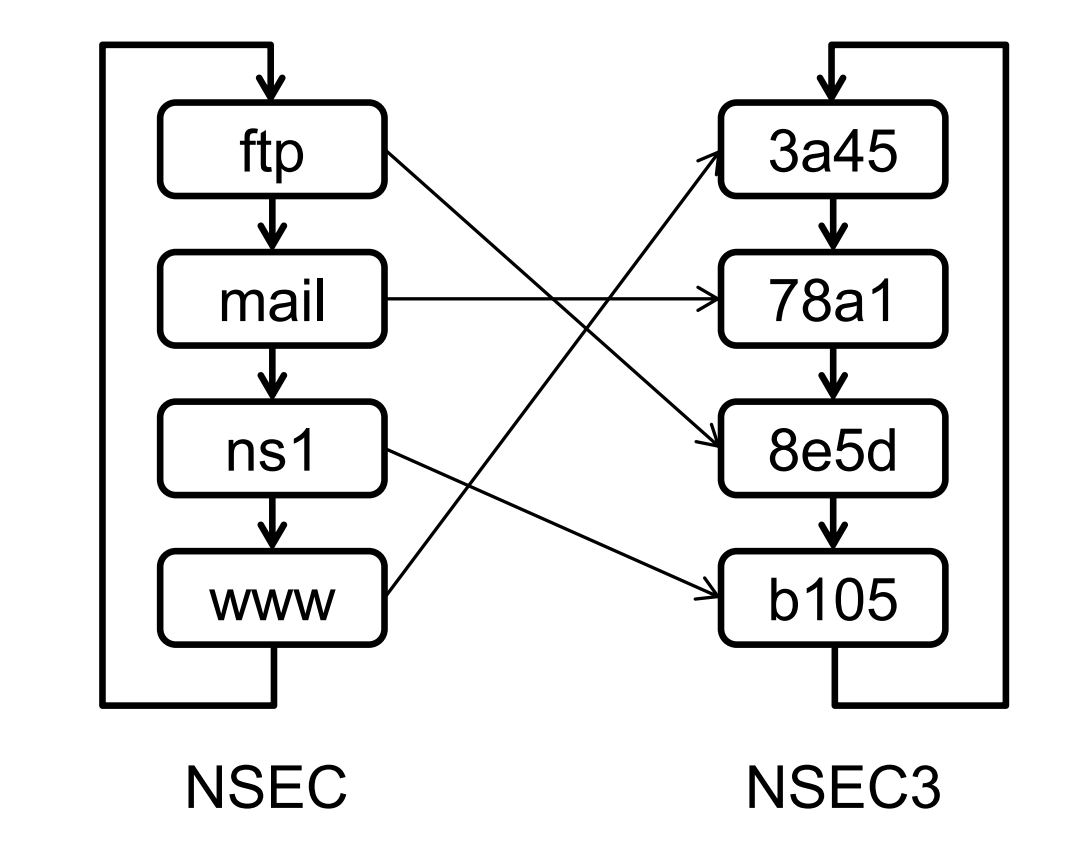
\includegraphics[width=0.5\textwidth]{nsec3.png}
    \caption{A simple representation of how NSEC and NSEC3 differ. In the canonical ordering NSEC uses a linked list of plaintext domain names in lexicographic order. NSEC uses a linked list of hashed domain name values. Image from \cite{NSEC3_hash_breaking}.} 
    \label{fig:hash_list}
  \end{center}
\end{figure}

Study conducted by \citet{NSEC3_hash_breaking} showed that even with NSEC3 zone enumeration is still possible using GPU-based NSEC hash breaking. The algorithm had two parts. Since querying NSEC3 records directly is impossible the first phase was to query non-existing random names until all NSEC3 records (or NSEC3 intervals) had been retrieved and NSEC3 intervals formed a fully connected and circular path so crawling NSEC3 intervals was finished.



After crawling the NSEC3 intervals brute forcing and dictionary based attack was used for hash breaking. The result was that approximately 64 \% of all NSEC3 hashes of the top level domain \texttt{com.} was reversed after 4.5 days of computation \cite{NSEC3_hash_breaking}. The Technique presented by \citet{NSEC3_hash_breaking} differs from using a brute force attack to directly query (or "bombard") a DNS server for domain names in a sense that the technique was carried out mostly offline. Notable is that the \texttt{com.} TLD NSEC3 hashing  used no salt in addition to zero iterations (hash computed only once) when computing the hash value for a domain name.


In addition in the study \citet{NSEC3_hash_breaking} learned that 52 \% of the TLDs did not change their salt value during the 1 year of observation period and 5 \% of the TLDs did not use salt at all making both cases vulnerable to "rainbow table" attacks i.e., table of precomputed hash values.

Since zone enumeration is feasible even with NSEC3, a variant of NSEC3, NSEC5 \cite{NSEC5} has been suggested to overcome the existing vulnerabilities in an authenticated denial of existence in NSEC and NSEC3. This thesis will not discuss NSEC5 but suffice to say that NSEC5 is designed so that it will prevent zone enumeration \cite{NSEC5_provably}. 
%https://www.ndss-symposium.org/wp-content/uploads/2017/09/06_5_0.pdf



\subsection{Subdomain enumeration}

The first stage in an attempt to enumerate subdomains is to try zone transfer attack but the probability of succeeding is low \cite{NSEC3_hash_breaking}. This section discusses the few methods which may be leveraged to enumerate subdomains. Enumeration of subdomains using methods described in this section can be used in conjunction with advanced search engine features e.g., “Google Dorks” to gather information about the subdomains \cite{hacking_exposed}.


\subsubsection{TTL/TLS certificates}

Information about subdomains can ge gathered by examining the TLS certificate for a top-level domain. A TLS certificate contains a field Certificate Subject Alternative Name which indicates all of the domain names and IP addresses that are covered by the certificate \citep{hacking_exposed}. As an example examining the certificate for \texttt{www.aalto.fi} one can see that the Subject Alternative Name field contains nearly 30 domain names:

\begin{verbatim}
DNS Name: aalto.fi
DNS Name: 5g-research.aalto.fi
DNS Name: abe.aalto.fi
DNS Name: accounting.aalto.fi
DNS Name: acre.aalto.fi
DNS Name: act.aalto.fi
DNS Name: aef.aalto.fi
DNS Name: aiic.aalto.fi
DNS Name: alumni.aalto.fi
...
DNS Name: www.aalto.fi
\end{verbatim}

Of course this is not a DNS enumeration technique per se but presents a simple yet effective way to enumerate subdomains in certain cases.

\subsubsection{Brute forcing}

As the name suggests simple dictionary based brute forcing for subdomains is not a very finessed method. On the other hand, the "guessing" of subdomain names is feasible to a certain degree since certain services tend to have names which reflect their purpose. The downside is that simplistic dictionary based brute forcing methods tend not to give reliable results since the method depend of a huge list of known words and
thus, will not work against unknown names \cite{SMART_BRUTE}. Most commonly known tools for enumerating subdomain names are \texttt{DNSEnum} \cite{dnsenum} and \texttt{Fierce} \cite{fierce} both using dictionary based brute forcing to enumerate subdomains in addition to methods described in previous sections.

\begin{figure}[h]
  \begin{center}
    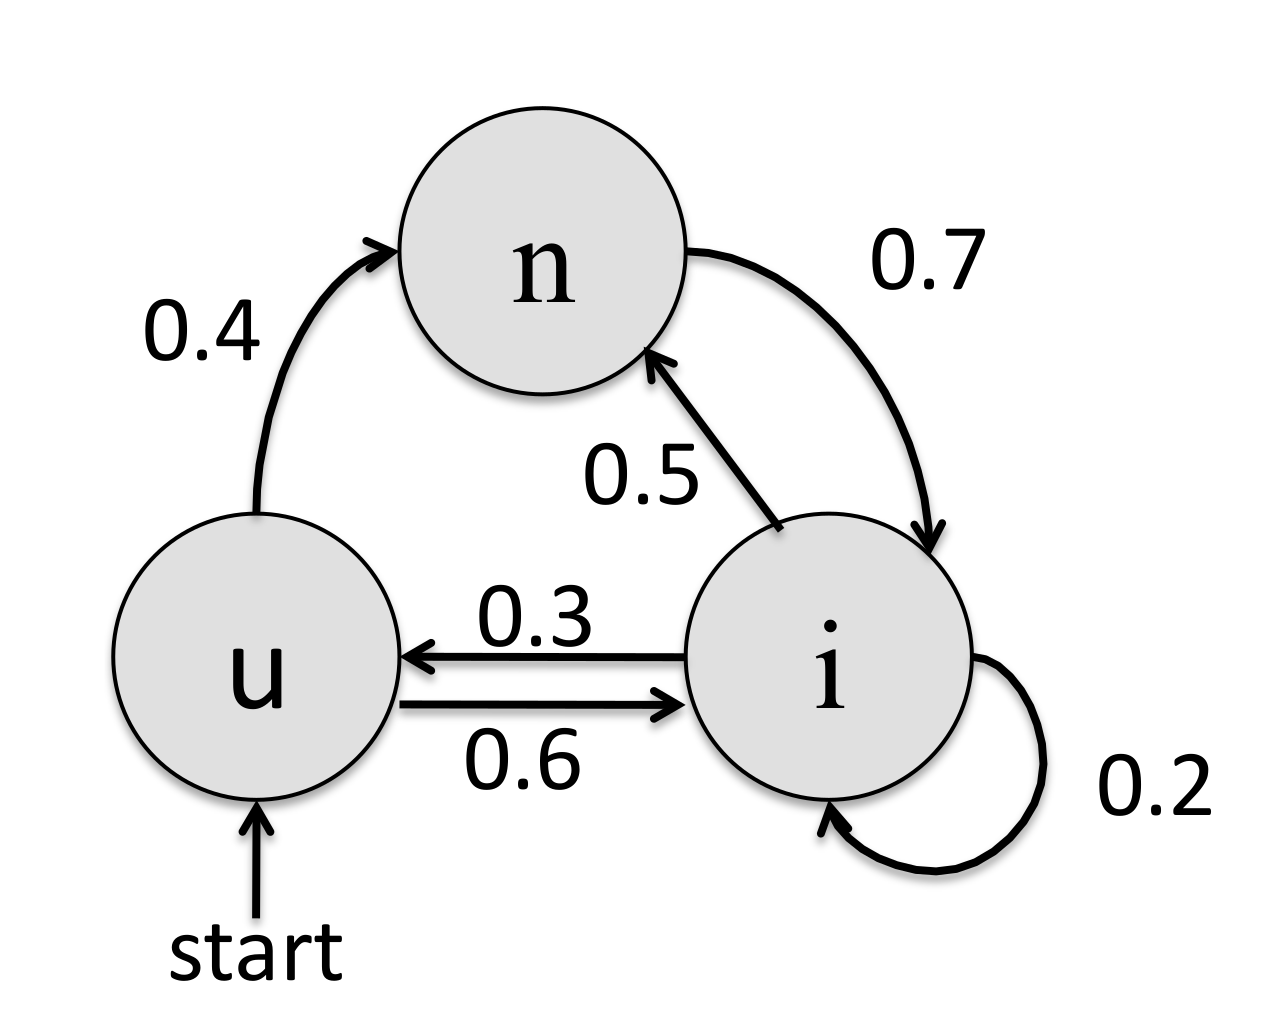
\includegraphics[width=0.3\textwidth]{markov.png}
    \caption{A simplistic illustration of generating subdomain names using a simple Markov chain model i.e., a state machine model. Using training data the transition probabilities were calculated by \citet{SMART_BRUTE} and the model was used to generate subdomain names. The initial character was chosen randomly based on the distribution of initial characters in the training data and subsequent characters were generated by the model.} 
    \label{fig:markov}
  \end{center}
\end{figure}

Instead using dictionary based attacks, \citet{SMART_BRUTE} demonstrated that applying a relatively simple language generation model achieved better results than a basic dictionary based brute forcing. The training data was gathered by passive DNS monitoring activity for generating the domain names, see Figure \ref{fig:markov} for more details.


The study conducted by \citet{SMART_BRUTE} is relatively old and one could argue that now fashionable autoregressive language models could be leveraged to generate subdomain names but no related studies were found.


\subsection{Enumerating Cloud Services}
\label{sec:cloud}

Services in the cloud may not reveal much information about the service as the internal infrastructure is not visible from outside. As an example, Figure \ref{fig:cloud_structure} illustrates a recommended three tier architecture for a cloud infrastructure in a case of Wordpress application in Amazon Web Services (AWS) \cite{AWSbestpractices}. In the architecture security critical components such as databases and volumes have been "hidden" in private subnets of the Virtual Private Cloud (VPC) with no access to the Internet thus making accessing and enumeration from the outside impossible. Enumeration of the internal structure would require the attacker to gain an access to an internal component such as an EC2 instance (virtual machine) in the case of AWS.

\begin{figure}[htb]
  \begin{center}
    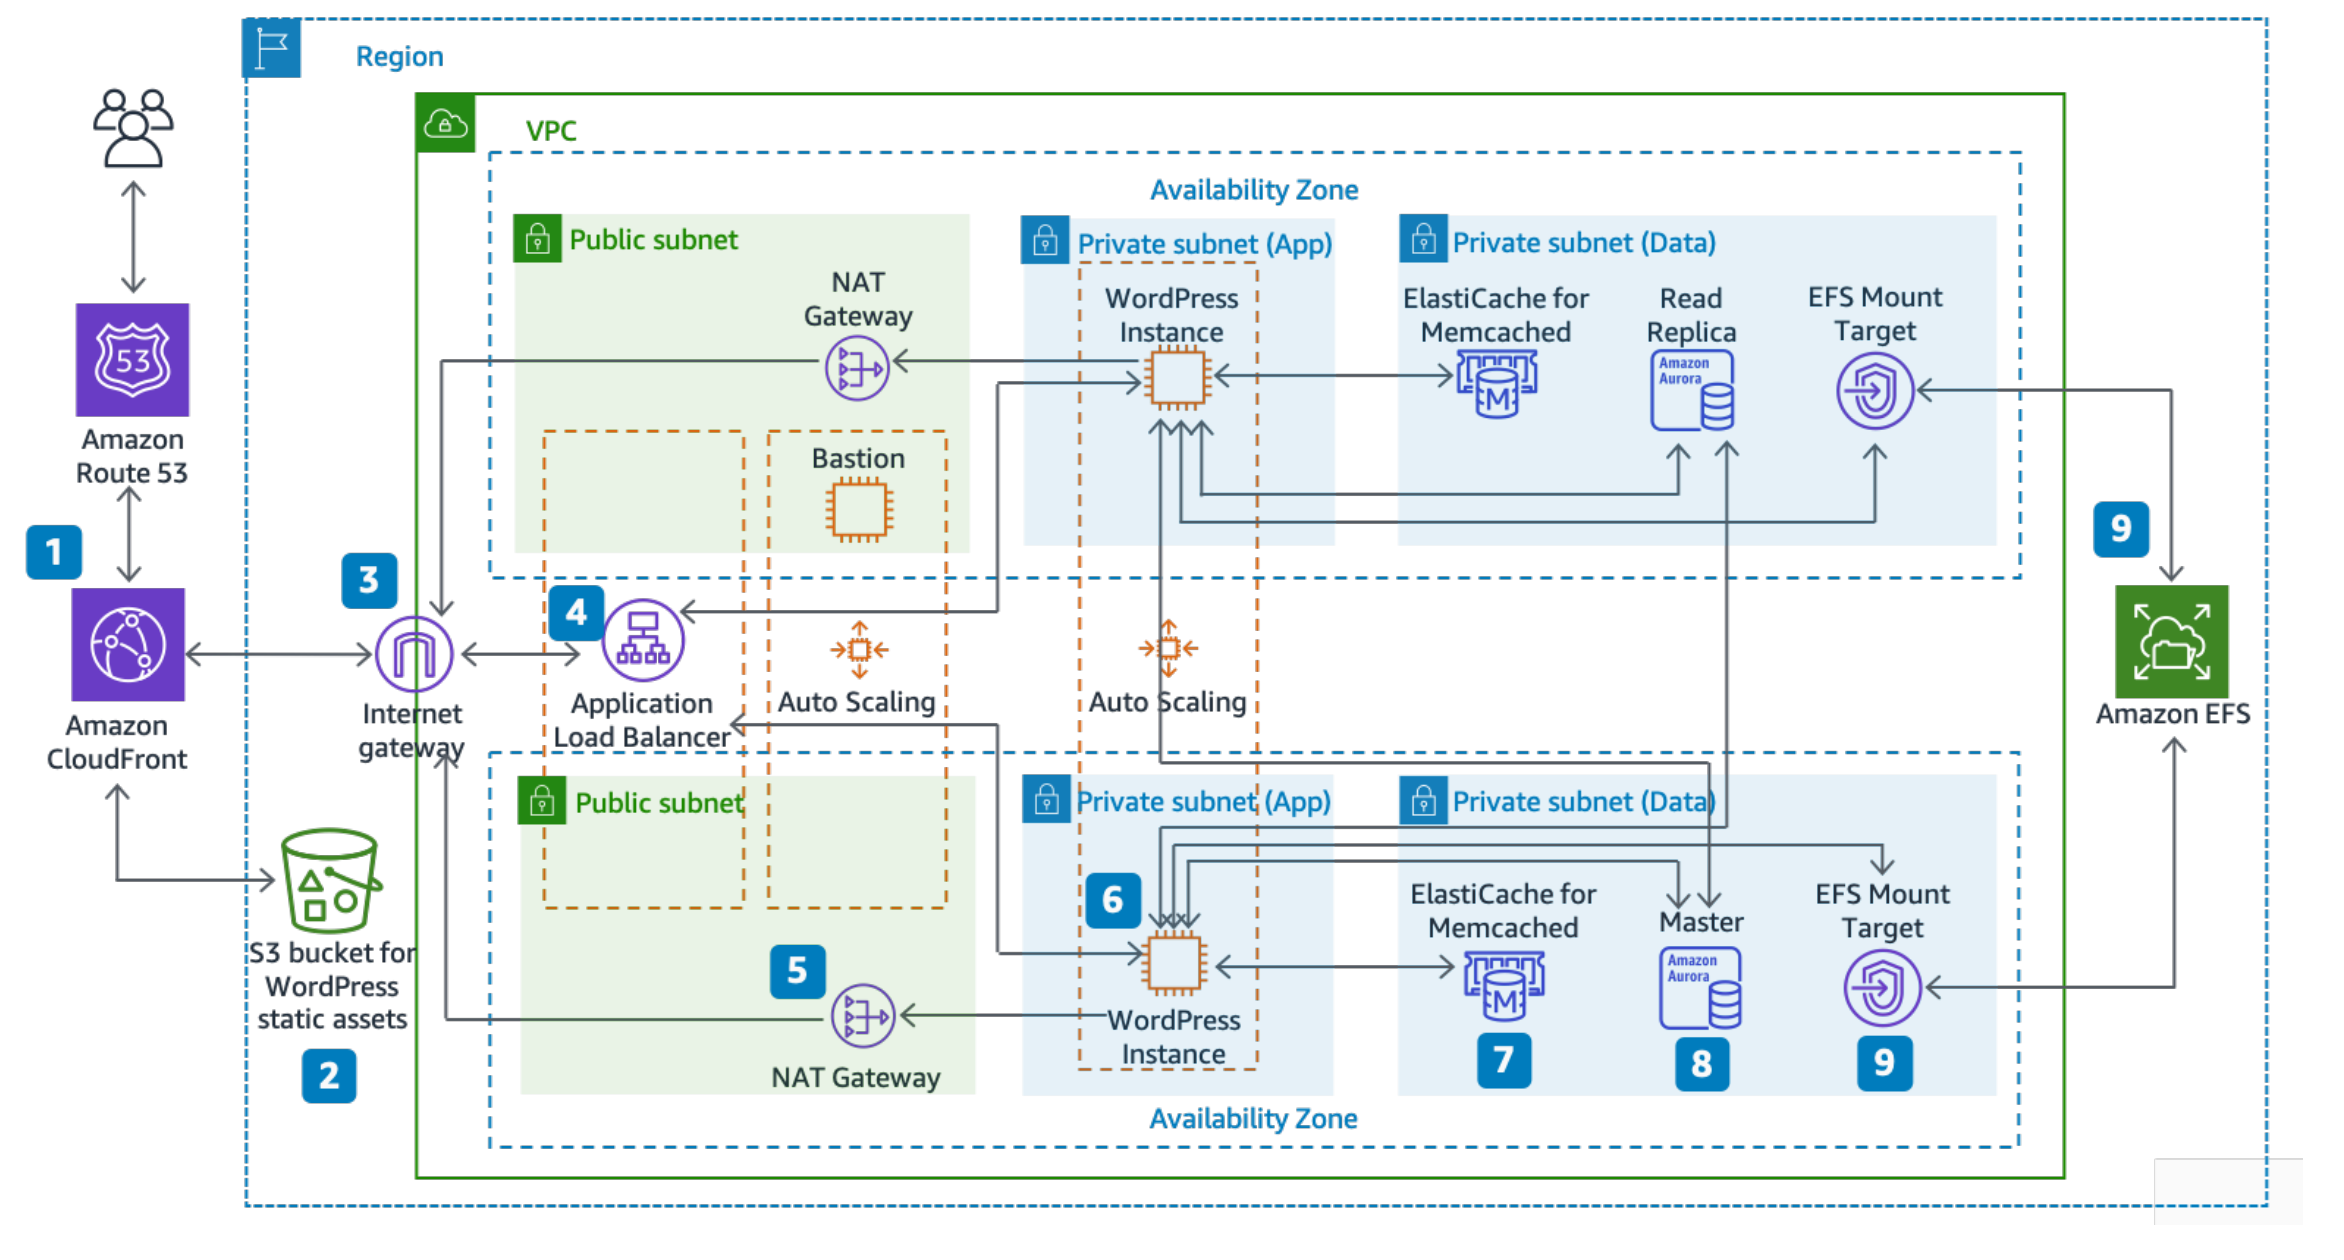
\includegraphics[width=1.0\textwidth]{cloud_rakenne.png}
    \caption{A three tier achitecture suggested by Amazon for a Wordpress application in Amazon Web Services \cite{AWSbestpractices}.} 
    \label{fig:cloud_structure}
  \end{center}
\end{figure}
For a content such as images for web sites or other uses for a storage AWS provides a service called Simple Storage System (S3) \cite{s3buckets}. Google Cloud platform offers a similar solution called Cloud Storage \cite{googlebuckets} both solutions being referred commonly as "buckets". The use of a bucket can range from serving static files for a web site to database backups.

Enumerating AWS S3 or Google Cloud Storage is popular as there are multiple AWS S3 and Google Cloud Storage enumerators available \cite{GCPBucket}\citep{AWSpentest}. Contents of a bucket may be configured to be either private or public. Many of the enumerators try to find misconfigured storages by brute forcing bucket names to find buckets in order to access information not intended to be public. Misconfigured buckets in some cases even allow a priviledge escalation attack \cite{GCPBucket}.

Using DNS queries to enumerate buckets in both cases is not possible. For Google Storage the domain name for accessing a bucket is the same for each of the buckets (\texttt{storage.googleapis.com} \cite{googlebuckets}) and path is used to access a specific bucket with a globally unique bucket name. All S3 buckets have a globally unique name as well and the domain name for a bucket is \texttt{<bucket-name>.s3.amazonaws.com} \cite{s3buckets}.

The latter gives a hint of a possibility to brute force buckets using DNS queries but this is not possible any more \cite{S3enum} since every DNS query for a non-existing bucket name returns a result which is indistinguishable  from a result for an existing bucket, possibly to prevent brute forcing using DNS queries. Instead enumerators available leverage either HTTP queries to bucket endpoints directly or use cloud provider command line interface software to query possible bucket names.

\section{Conclusion and Future Work}

The Domain Name System is an integral and critical part of the Internet infrastructure and without it the Internet would be considerably less user friendly. The Domain Name System originates from a time when the Internet was relatively new and there was not much emphasis on security. The DNS has a long history of being vulnerable to cache poisoning and DDoS attacks and still to this day the DNS traffic is unencrypted which allows passive information gathering. In addition to being vulnerable to cyber attacks such as cache poisoning, publicity of DNS records allows enumerating target network infrastructure.

Later on the different security measures to DNS have been introduced. Transmission signatures or TSIG use shared private keys to provide authentication of servers to secure actions such as zone transfers and dynamic updates of resource records. DNS Security Extensions or DNSSEC have been introduced early on to provide end-to-end data integrity and source authenticity check between the source of DNS data and the client but the adoption process is still underway. Interestingly, DNSSEC opened up a possibility for a new kind of DNS enumeration technique called Zone Walking. Zone walking was not originally considered a security threat but later on a consensus was reached that enabling a possibility to enumerate the whole DNS zone using DNSSEC records was an undesirable feature. NSEC3 was introduced to make zone walking considerably harder but due to the increase of computing power and its easy access, NSEC3 turned out to be vulnerable to zone walking, thus NSEC5 has been proposed.

The DNS enumaration methods discussed are methods are Zone Transfer Attack, reverse DNS sweeping, Zone Walking and brute forcing subdomain names. If the Zone Transfer attack fails - which usually is the case - there's no guarantee that an attacker can map the whole target infrastructure especially in case of enumeration of subdomain names. But in addition to "traditional" DNS enumeration methods, attacker can use other methods in conjuction such as advanced search engine features and inspecting TLS certificates for a certain domain. The most comprehensive result is achieved by using multiple methods.

Even though this thesis discussed how to use DNS enumeration techniques to query DNS servers, an attacker does not have to query DNS servers directly. There are online resources that keep records of domains and their subdomains. The information available has been gathered using multiple different methods described in this study.

The focus of this study has been "traditional" DNS enumeration. Since services move to the cloud and services may consist of multiple microservices this opens up new possibilities to leverage DNS or more generally service enumeration techniques. As discussed in the Chapter \ref{sec:cloud} from outside services may not reveal much information but if an attacker gains a foothold in the system e.g., Kubernetes cluster, EC2 instance of Amazon Web Services or a Compute Engine instance of Google Cloud Platform, this opens up new ways for enumerating services from the inside. Unfortunately discussing this aspect was not possible due to the time restrictions but it would be an interesting topic for a further study.


% --------------------------------------------------------------------
